% Author: Lam Chi Hao
% Author: Vo Nhat Tien
% Author: Le Nguyen Anh Tri
% Last update: 23/11/2024

\documentclass[12pt]{article}
<<<<<<< HEAD
=======
\usepackage{tikz}
>>>>>>> master
\usepackage{amsmath}
\usepackage{amsfonts}
\usepackage{pdflscape}
\usepackage{fancyhdr}
<<<<<<< HEAD
=======
\usepackage{ulem}
>>>>>>> master
\usepackage{graphicx}
\usepackage[colorlinks = true,
            linkcolor = magenta,
            urlcolor = magenta,
            citecolor = magenta,
            anchorcolor = magenta]{hyperref}
\usepackage{url}
\usepackage[top = .75in, left = .75in, right = .75in, bottom = 1in]{geometry}

% Table
\usepackage{array}

% For algorithm
\usepackage{algorithm}
\usepackage{algpseudocode}

% For code
\usepackage{listings}
\usepackage{xcolor}
\definecolor{codegreen}{rgb}{0, 0.6, 0}
\definecolor{codegray}{rgb}{0.5, 0.5, 0.5}
\definecolor{codepurple}{rgb}{0.58, 0, 0.82}
\definecolor{backcolour}{rgb}{0.95, 0.95, 0.92}

\lstdefinestyle{mystyle} {
    backgroundcolor = \color{backcolour},
    commentstyle = \color{codegreen},
    keywordstyle = \color{magenta},
    numberstyle = \tiny\color{codegray},
    stringstyle = \color{codepurple},
    basicstyle = \ttfamily\footnotesize,
    breakatwhitespace = false,
    breaklines = true,
    captionpos = b,
    keepspaces = true,
    numbers = left,
    numbersep = 5pt,
    showspaces = false,
    showstringspaces = false,
    showtabs = false,
    tabsize = 2
}
\lstset{style = mystyle}

\setlength{\parindent}{0pt}

\newcommand{\coursename}{Fundamentals of Programming}
\newcommand{\reportname}{Final Project}
\newcommand{\reporttitle}{Poker Game}

\newcommand{\studentname}{Lam Chi Hao \\ Vo Nhat Tien \\ Le Nguyen Anh Tri}
\newcommand{\teachername}{Nguyen Hai Minh \\ Tran Thi Thao Nhi \\ Phan Thi Phuong Uyen}


% ============ HEADER AND FOOTER ============
% Header length
\setlength{\headheight}{29.43912pt}

% Footer page number would be on the lower-right corner
\pagestyle{fancy}
\fancyfoot{}
\fancyfoot[R]{Page \thepage}

\lhead{\reporttitle}
\rhead{\coursename}

%\lfoot{\leftfooter}
\renewcommand{\footrulewidth}{0.4pt}
\lfoot{University of Science - VNU-HCM}

% Footer page number for landscape
\fancypagestyle{lscape}{
\fancyhf{}
\fancyfoot[R]{Page\thepage}
\renewcommand{\headrulewidth}{0pt} 
\renewcommand{\footrulewidth}{0pt}
}

%Document
\begin{document}

% Cover paper
% Description: Cover paper of the report.

\begin{titlepage}
    
    \newcommand{\HRule}{\rule{\linewidth}{0.5mm}}
    \centering
    
    \textsc{\LARGE viet nam national university ho chi minh city}\\ [0.5cm]
    \textsc{\large university of science} \\ [0.5cm]
    \textsc{\large faculty of information technology} \\ [0.5cm]
    
    % HCMUS Logo and report title
    
\includegraphics[scale = 0.36]{figures/hcmus-logo.jpeg} \\ [0cm]
    \HRule \\ [0.2cm]
    {
    \huge{\bfseries{\reporttitle}}\\[0.2cm]
    \Large{\bfseries{Report Name: \reportname}}
    }
    \\[0.2cm]
    \HRule \\ [0.2cm]
    
    \textbf{\large Course name: \coursename}\\ [0.3cm]
    \textbf{\large CSC1002 - 24C03} \\ [1.3cm]
    
    % Student and teacher name
    \begin{minipage}[t]{0.4\textwidth}
    \begin{flushleft} \large
    \emph{Student name: }\\
    \studentname
    \end{flushleft}
    \end{minipage}
    ~
    \begin{minipage}[t]{0.4\textwidth}
    \begin{flushright} \Large
    \emph{Teacher name: } \\
    \teachername
    \end{flushright}
    \end{minipage} \\[4.2cm]
    % TODO: Add date of submission.
    {\large \today} \\[0.4cm]
    \vfill
    
\end{titlepage}

\tableofcontents
\pagebreak

% Information group page
% Description: Information of group members.
\section{Group Information}
\label{sec:group-information}

\renewcommand{\arraystretch}{1.5}
\begin{table}[ht]
    \centering
    \begin{tabular}{| m{1.75cm} | m{2cm} | m{5cm}| m{2.5cm} |} 
    \hline
    \textbf{} & \textbf{ID} & \textbf{Name} & \textbf{Title} \\ 
    \hline
    1 & 24127034 & Lam Chi Hao & Leader \\ 
    \hline
    2 & 24127557 & Vo Nhat Tien & Member \\ 
    \hline
    3 & 24127567 & Le Nguyen Anh Tri & Member \\ 
    \hline
    \end{tabular}
    \caption{Information of Group 02 member.}
    \label{tab:group-information}
\end{table}

% Table of contribution
% Description: Table of contribution
\section{Table of Contribution}
<<<<<<< HEAD
\label{sec:table-of-contribution}
=======
\label{sec:contribution-table}
>>>>>>> master

% TODO: Fill the table
\renewcommand{\arraystretch}{1.5} % Tăng chiều cao hàng
\begin{table}[ht]
    \centering
    \begin{tabular}{|m{4cm}|m{2cm}|m{2cm}|m{2cm}| m{2cm}|}
    \hline
    \textbf{Problem} & \textbf{Rubric} & \textbf{24127034} & \textbf{24127557} & \textbf{24127567} \\
    \hline
    Standard features & - &  &  &  \\
    \hline
<<<<<<< HEAD
    Initialization & 20 & Score & Score & Score \\
    \hline
    Dealing & 20 & Score & Score & Score \\
    \hline 
    Game play & 20 & Score & Score & Score \\
    \hline
    Player's information & 20 & Score & Score & Score \\
    \hline
    Advanced features & - &  &  &  \\
    \hline 
    Draw poker & 30 & Score & Score & Score \\
    \hline
    5-card stud & 30 & Score & Score & Score \\
    \hline
    Color / Sound effects & 30 & Score & Score & Score \\
=======
    Initialization & 20 & 15 & 0 & 5 \\
    \hline
    Dealing & 20 & 5 & 0 & 15 \\
    \hline 
    Game play & 20 & 0 & 0 & 20 \\
    \hline
    Player's information & 20 & 5 & 0 & 15 \\
    \hline
    Advanced features & - &  &  &  \\
    \hline 
    Draw poker & 30 & 0 & 0 & 30 \\
    \hline
    5-card stud & 30 & Score & Score & Score \\
    \hline
    Color / Sound effects & 30 & 30 & 0 & 0 \\
>>>>>>> master
    \hline
    Leader board & 30 & Score & Score & Score \\
    \hline
    Creations & 30 / each & Score & Score & Score \\
    \hline
    Report & - &  &  &  \\
    \hline
<<<<<<< HEAD
     & 100 & Score & Score & Score \\
    \hline
    & Total & Score & Score & Score \\
    \hline
    \end{tabular}
    \caption{Table of contribution}
    \label{tab:table-of-contribution}
=======
     & 100 & 10 & 0 & 0 \\
    \hline
    & Total & 65 & 0 & 85 \\
    \hline
    \end{tabular}
    \caption{Table of contribution}
    \label{tab:contribution-table}
>>>>>>> master

\end{table}

<<<<<<< HEAD
% References
% Description: Contains the list of references.
\section{List of References}
<<<<<<< HEAD
\label{sec:list-of-references}
=======
\label{sec:references-list}
>>>>>>> master

% TODO: Fill the references
\begin{itemize}
    \item \LaTeX \space template: \url{https://github.com/khongsomeo/hcmus-unofficial-report-template}.
    \item \LaTeX \space on Visual Studio Code tutorial: \url{https://youtu.be/4lyHIQl4VM8}.
\end{itemize}

% Report contents
=======
% Acknowledgement
\section{Acknowledgement}
\label{sec:acknowledgment-section}

\hspace{1cm} We would like to sincerely thank our theory teacher, Nguyen Hai Minh, and our lab teachers, Nguyen Thi Thao Nhi and Phan Thi Phuong Uyen, for providing the project and valuable resources for self-studying. Although their guidance was indirect, the materials helped us understand the fundamental concepts needed for this project.

\vspace{0.5cm}

\hspace{1cm} We first consisted of a team of three; however, one of our teammates did not feel this was the correct field for him and left our team. Despite the obstacle that challenged us, we tried our best to give our best effort to finish the project.

\vspace{0.5cm}

\hspace{1cm} We consider ourselves very lucky that this opportunity for the project was given to us and allowed us to learn by experience. Any limitations or shortcomings in this work are entirely our responsibility. We hope that this project will be a stepping stone for us to improve our skills and knowledge in the future.

% Report contents
\section{Introduction}
\label{sec:introduction}

\hspace{1cm} This report is our final report of the project \textit{Poker Game} for the course \textit{Fundamentals of Programming - CSC10012}. The project is a poker game application that allows users to play poker with the computer and other players locally. The game is developed using C++ programming language and SDL2 library for graphical user interface. The project is divided into two main parts: core mechanics and graphical user interface. The core mechanics of the game are implemented using classes and structures.

\vspace{0.5cm}

\hspace{1cm} TODO: Add more information about the project

\vspace{0.5cm}

\hspace{1cm} The report provides an overview of the project, including the project structure, the flowchart of the game, the structure of the game using SDL2 library, the implementation of the game, and the conclusion.

% End of Introduction.tex
\section{Project Structure}
\label{sec:project-structure-section}

\hspace{1cm} For this part of the report, we will discuss the project structure, including the folder structure, file structure, variable, constant, class, and structure naming conventions. 

\vspace{0.5cm}

\hspace{1cm} The naming convention is a set of rules for choosing the character sequence to represent the name of a variable, constant, function, class, file, folder, or other entity in the source code. The naming convention is essential because it helps the reader understand the code more easily and quickly. In this project, we follow the naming convention below:

\subsection{Folder Structure}
\begin{itemize}
    \item \textbf{Lowercase}: All characters in the folder name are lowercase.
    \item \textbf{Underscore}: If the folder name consists of multiple words, separate them with an underscore.
\end{itemize}

Our folder structure is as follows:
\begin{itemize}
    \item \textbf{src}: Contains all source code files written in C++. There are two subfolders with two main categories of source code files.
    \begin{itemize}
        \item \textbf{core}: Contains all the source files relate to the core mechanics of the game.
        \item \textbf{gui}: Contains all the source files relate to graphical user interface of the game.
    \end{itemize}
    \item \textbf{include}: Contains all header files. There are two subfolders with two main categories of header files.
    \begin{itemize}
        \item \textbf{core}: Contains all the header files relate to the core mechanics of the game.
        \item \textbf{gui}: Contains all the header files relate to graphical user interface of the game.
    \end{itemize}
    \item \textbf{bin}: Contains all executable files, object files and dynamic libraries. There is a subfolder called obj. Inside the obj folder, there are two subfolders with two main categories of object files.
    \begin{itemize}
        \item \textbf{core}: Contains all the object files relate to the core mechanics of the game.
        \item \textbf{gui}: Contains all the object files relate to graphical user interface of the game.
    \end{itemize}
    \item \textbf{assets}: Contains all assets used in the project. There are three subfolders inside our assets folder.
    \begin{itemize}
        \item \textbf{imgs}: Contains all images used in the project. There are imgs for backgrounds, buttons, cards, cursor and icons for our game application.
        \item \textbf{audios}: Contains all sounds used in the project. There are audios for background music, button click sound, card shuffle sound and card flip sound.
        \item \textbf{fonts}: Contains all fonts used in the project. There are fonts for the game title, game buttons and game text.
    \end{itemize}
    \item \textbf{libs}: Contains all libraries used in the project.
    \begin{itemize}
        \item \textbf{SDL2}: Contains all SDL2 libraries. This is our main library for creating the graphical user interface.
        \item \textbf{cmake}: Contains all CMake libraries.
    \end{itemize}
    \item \textbf{report}: Contains all report files which are source code files written in LaTeX.
    \begin{itemize}
        \item \textbf{contents}: Contains all the contents of the report. We want to keep the report organized, so we separate the report into multiple files and put them in the contents folder.
        \item \textbf{figures}: Contains all figures used in the report. The figures are images, graphs, tables, etc.
    \end{itemize}
\end{itemize}

\subsection{File Structure}
\begin{itemize}
    \item \textbf{lowercase}: Only one exception is our main file, which is named \textbf{main.cpp}.
    \item \textbf{CamelCase}: We decide that all of the header files and source files are named in CamelCase.
    \item \textbf{Underscore \& hyphen}: This is for files in SDL2 libraries, which are named in lowercase and separated by an underscore. Beside that, our files in assets are named in lowercase and separated by an underscore or hyphen.
\end{itemize}

\subsection{Variable, constant, class, structure}
\begin{itemize}
    \item \textbf{camelCase}: We decide that all of the variables are named in camelCase. Notice that the first letter of the first word is lowercase, and the first letter of the following words is uppercase.
    \item \textbf{CamelCase}: For classes and structures in our project, we decide that all of the classes and structures are named in CamelCase. Notice that the first letter of each word is uppercase.
    \item \textbf{ALL CAPS}: We decide that all of the constants are named in ALL CAPS. Notice that if the constant consists of multiple words, we will separate them with an underscore.
\end{itemize}

\subsection{Function Prototype and Definition}
\hspace{1cm} We decide that all of the functions are named in camelCase. Notice that the first letter of the first word is lowercase, and the first letter of the following words is uppercase.
\section{Chart}
\label{sec:chart}

\hspace{1cm} This part will provide a chart of the project's structure. The chart will show the relationship between the classes and the functions of the project. The chart will be divided into two parts: the first part will show the relationship between the classes, and the second part will show the functions of the project.

\vspace{0.5cm}

\hspace{1cm} TODO: Write more about the chart of the project's structure

\subsection{Core class relationship}

\hspace{1cm} TODO: Write more about the class relationship

\vspace{0.5cm}

\hspace{1cm} TODO: Add the chart of the class relationship

\subsection{GUI function relationship}

\hspace{1cm} TODO: Write more about the function relationship

\vspace{0.5cm}

\hspace{1cm} TODO: Add the chart of the function relationship

\subsection{Program flowchart}

\hspace{1cm} TODO: Write more about the program flowchart

% End of Chart.tex

\section{SDL2 Game Structure}
\label{sec:SDL2-Game-Structure-section}

% Give me the basic structure of the game using SDL2
In this section, we will explore the fundamental structure of our SDL2-based poker game. The game follows a standard SDL2 application architecture with the following key components:

\begin{itemize}
    \item \textbf{Initialization}: Setting up SDL2, creating windows and renderers
    \item \textbf{Game Loop}: The main loop that handles:
        \begin{itemize}
            \item Event handling (user input)
            \item Game state updates
            \item Rendering
        \end{itemize}
    \item \textbf{Resource Management}: Loading and managing textures, fonts, and sounds
    \item \textbf{Cleanup}: Proper deallocation of resources
\end{itemize}

\subsection{Core Components}
The game is structured around several core classes:

\begin{itemize}
    \item \texttt{Game}: Main class managing the game state and loop
    \item \texttt{TextureManager}: Handles loading and rendering of images
    \item \texttt{InputHandler}: Processes user input
    \item \texttt{Player}: Manages player data and actions
    \item \texttt{Card}: Represents individual playing cards
    \item \texttt{Deck}: Handles the deck of cards and dealing
\end{itemize}

Figure \ref{fig:game-structure} illustrates the relationship between these components.

\begin{figure}[h]
    \centering
    \begin{tikzpicture}[node distance=2cm]
        \node[rectangle,draw] (game) {Game};
        \node[rectangle,draw] (texture) [below left of=game] {TextureManager};
        \node[rectangle,draw] (input) [below of=game] {InputHandler};
        \node[rectangle,draw] (player) [below right of=game] {Player};
        
        \draw[->] (game) -- (texture);
        \draw[->] (game) -- (input);
        \draw[->] (game) -- (player);
    \end{tikzpicture}
    \caption{Basic game structure diagram}
    \label{fig:game-structure}
\end{figure}


\section{Implementation}
\label{sec:implementation}

\hspace{1cm} The implementation of the project is divided into two main parts: core mechanics and graphical user interface. The core mechanics of the game are implemented using classes and structures. The graphical user interface is implemented using the SDL2 library. The project is developed using C++ programming language.

\subsection{Core Mechanics}
\label{subsec:core-mechanics}

\hspace{1cm} The core mechanics of the game are implemented using classes and structures. The core classes of the project are \texttt{Game}, \texttt{Player}, \texttt{Card}, and \texttt{Deck}. The \texttt{Game} class manages the game state and loop. The \texttt{Player} class manages player data and actions. The \texttt{Card} class represents individual playing cards. The \texttt{Deck} class handles the deck of cards and dealing.

\vspace{0.5cm}

\begin{itemize}
    \item \textbf{Game}: Main class managing the game state and loop
    \item \textbf{Player}: Manages player data and actions
    \item \textbf{Card}: Represents individual playing cards
    \item \textbf{Deck}: Handles the deck of cards and dealing
\end{itemize}

\vspace{0.5cm}
\input{contents/Conclusion.tex}
\input{contents/FutureWork.tex}


% References
% Description: Contains the list of references.
\section{List of References}
<<<<<<< HEAD
\label{sec:list-of-references}
=======
\label{sec:references-list}
>>>>>>> master

% TODO: Fill the references
\begin{itemize}
    \item \LaTeX \space template: \url{https://github.com/khongsomeo/hcmus-unofficial-report-template}.
    \item \LaTeX \space on Visual Studio Code tutorial: \url{https://youtu.be/4lyHIQl4VM8}.
\end{itemize}

>>>>>>> master

\end{document}